\documentclass[12pt,openany]{book}
\usepackage{lmodern}
\usepackage{amssymb,amsmath}
\usepackage{ifxetex,ifluatex}
\usepackage{fixltx2e} % provides \textsubscript
\ifnum 0\ifxetex 1\fi\ifluatex 1\fi=0 % if pdftex
  \usepackage[T1]{fontenc}
  \usepackage[utf8]{inputenc}
\else % if luatex or xelatex
  \ifxetex
    \usepackage{mathspec}
  \else
    \usepackage{fontspec}
  \fi
  \defaultfontfeatures{Ligatures=TeX,Scale=MatchLowercase}
    \setmonofont[Mapping=tex-ansi,Scale=0.8]{Source Code Pro}
\fi
% use upquote if available, for straight quotes in verbatim environments
\IfFileExists{upquote.sty}{\usepackage{upquote}}{}
% use microtype if available
\IfFileExists{microtype.sty}{%
\usepackage{microtype}
\UseMicrotypeSet[protrusion]{basicmath} % disable protrusion for tt fonts
}{}
\usepackage[margin=1in]{geometry}
\usepackage{hyperref}
\hypersetup{unicode=true,
            pdftitle={Machine Learning for Biological Sciences},
            pdfauthor={Vincent Wu},
            pdfborder={0 0 0},
            breaklinks=true}
\urlstyle{same}  % don't use monospace font for urls
\usepackage{natbib}
\bibliographystyle{apalike}
\usepackage{color}
\usepackage{fancyvrb}
\newcommand{\VerbBar}{|}
\newcommand{\VERB}{\Verb[commandchars=\\\{\}]}
\DefineVerbatimEnvironment{Highlighting}{Verbatim}{commandchars=\\\{\}}
% Add ',fontsize=\small' for more characters per line
\usepackage{framed}
\definecolor{shadecolor}{RGB}{248,248,248}
\newenvironment{Shaded}{\begin{snugshade}}{\end{snugshade}}
\newcommand{\KeywordTok}[1]{\textcolor[rgb]{0.13,0.29,0.53}{\textbf{#1}}}
\newcommand{\DataTypeTok}[1]{\textcolor[rgb]{0.13,0.29,0.53}{#1}}
\newcommand{\DecValTok}[1]{\textcolor[rgb]{0.00,0.00,0.81}{#1}}
\newcommand{\BaseNTok}[1]{\textcolor[rgb]{0.00,0.00,0.81}{#1}}
\newcommand{\FloatTok}[1]{\textcolor[rgb]{0.00,0.00,0.81}{#1}}
\newcommand{\ConstantTok}[1]{\textcolor[rgb]{0.00,0.00,0.00}{#1}}
\newcommand{\CharTok}[1]{\textcolor[rgb]{0.31,0.60,0.02}{#1}}
\newcommand{\SpecialCharTok}[1]{\textcolor[rgb]{0.00,0.00,0.00}{#1}}
\newcommand{\StringTok}[1]{\textcolor[rgb]{0.31,0.60,0.02}{#1}}
\newcommand{\VerbatimStringTok}[1]{\textcolor[rgb]{0.31,0.60,0.02}{#1}}
\newcommand{\SpecialStringTok}[1]{\textcolor[rgb]{0.31,0.60,0.02}{#1}}
\newcommand{\ImportTok}[1]{#1}
\newcommand{\CommentTok}[1]{\textcolor[rgb]{0.56,0.35,0.01}{\textit{#1}}}
\newcommand{\DocumentationTok}[1]{\textcolor[rgb]{0.56,0.35,0.01}{\textbf{\textit{#1}}}}
\newcommand{\AnnotationTok}[1]{\textcolor[rgb]{0.56,0.35,0.01}{\textbf{\textit{#1}}}}
\newcommand{\CommentVarTok}[1]{\textcolor[rgb]{0.56,0.35,0.01}{\textbf{\textit{#1}}}}
\newcommand{\OtherTok}[1]{\textcolor[rgb]{0.56,0.35,0.01}{#1}}
\newcommand{\FunctionTok}[1]{\textcolor[rgb]{0.00,0.00,0.00}{#1}}
\newcommand{\VariableTok}[1]{\textcolor[rgb]{0.00,0.00,0.00}{#1}}
\newcommand{\ControlFlowTok}[1]{\textcolor[rgb]{0.13,0.29,0.53}{\textbf{#1}}}
\newcommand{\OperatorTok}[1]{\textcolor[rgb]{0.81,0.36,0.00}{\textbf{#1}}}
\newcommand{\BuiltInTok}[1]{#1}
\newcommand{\ExtensionTok}[1]{#1}
\newcommand{\PreprocessorTok}[1]{\textcolor[rgb]{0.56,0.35,0.01}{\textit{#1}}}
\newcommand{\AttributeTok}[1]{\textcolor[rgb]{0.77,0.63,0.00}{#1}}
\newcommand{\RegionMarkerTok}[1]{#1}
\newcommand{\InformationTok}[1]{\textcolor[rgb]{0.56,0.35,0.01}{\textbf{\textit{#1}}}}
\newcommand{\WarningTok}[1]{\textcolor[rgb]{0.56,0.35,0.01}{\textbf{\textit{#1}}}}
\newcommand{\AlertTok}[1]{\textcolor[rgb]{0.94,0.16,0.16}{#1}}
\newcommand{\ErrorTok}[1]{\textcolor[rgb]{0.64,0.00,0.00}{\textbf{#1}}}
\newcommand{\NormalTok}[1]{#1}
\usepackage{longtable,booktabs}
\usepackage{graphicx,grffile}
\makeatletter
\def\maxwidth{\ifdim\Gin@nat@width>\linewidth\linewidth\else\Gin@nat@width\fi}
\def\maxheight{\ifdim\Gin@nat@height>\textheight\textheight\else\Gin@nat@height\fi}
\makeatother
% Scale images if necessary, so that they will not overflow the page
% margins by default, and it is still possible to overwrite the defaults
% using explicit options in \includegraphics[width, height, ...]{}
\setkeys{Gin}{width=\maxwidth,height=\maxheight,keepaspectratio}
\IfFileExists{parskip.sty}{%
\usepackage{parskip}
}{% else
\setlength{\parindent}{0pt}
\setlength{\parskip}{6pt plus 2pt minus 1pt}
}
\setlength{\emergencystretch}{3em}  % prevent overfull lines
\providecommand{\tightlist}{%
  \setlength{\itemsep}{0pt}\setlength{\parskip}{0pt}}
\setcounter{secnumdepth}{5}
% Redefines (sub)paragraphs to behave more like sections
\ifx\paragraph\undefined\else
\let\oldparagraph\paragraph
\renewcommand{\paragraph}[1]{\oldparagraph{#1}\mbox{}}
\fi
\ifx\subparagraph\undefined\else
\let\oldsubparagraph\subparagraph
\renewcommand{\subparagraph}[1]{\oldsubparagraph{#1}\mbox{}}
\fi

%%% Use protect on footnotes to avoid problems with footnotes in titles
\let\rmarkdownfootnote\footnote%
\def\footnote{\protect\rmarkdownfootnote}

%%% Change title format to be more compact
\usepackage{titling}

% Create subtitle command for use in maketitle
\newcommand{\subtitle}[1]{
  \posttitle{
    \begin{center}\large#1\end{center}
    }
}

\setlength{\droptitle}{-2em}

  \title{Machine Learning for Biological Sciences}
    \pretitle{\vspace{\droptitle}\centering\huge}
  \posttitle{\par}
    \author{Vincent Wu}
    \preauthor{\centering\large\emph}
  \postauthor{\par}
      \predate{\centering\large\emph}
  \postdate{\par}
    \date{2018-12-10}

\usepackage{booktabs}

\begin{document}
\maketitle

{
\setcounter{tocdepth}{1}
\tableofcontents
}
\chapter{Foreword}\label{foreword}

This book is written and compiled using the \texttt{bookdown} package
for the R statistical language. Sections of this book will feature code
and graphs produced using R as well. As will be discussed in the next
chapter, the purpose of this paper is to introduce and broadly cover
common machine learning techniques that are used in the biological
sciences. Any included R code is for generating graphs and results to
provide additional content in conveying the different techniques. As
such, I opted to include the R code as a starting point for any readers
who want to explore the techniques.

The following code in this chapter are needed to load in additional
software packages and to load in the data that will be used in the later
chapters.

\begin{Shaded}
\begin{Highlighting}[]
\KeywordTok{library}\NormalTok{(tidyverse)}
\KeywordTok{library}\NormalTok{(usedist)}
\KeywordTok{library}\NormalTok{(qiimer)}
\KeywordTok{library}\NormalTok{(reshape2)}
\KeywordTok{library}\NormalTok{(ggplot2)}

\KeywordTok{library}\NormalTok{(ape)}
\KeywordTok{library}\NormalTok{(tree)}
\KeywordTok{library}\NormalTok{(Rtsne)}
\KeywordTok{library}\NormalTok{(class)}
\KeywordTok{library}\NormalTok{(randomForest)}
\KeywordTok{library}\NormalTok{(e1071)}
\KeywordTok{library}\NormalTok{(cluster)}
\end{Highlighting}
\end{Shaded}

\begin{Shaded}
\begin{Highlighting}[]
\KeywordTok{load}\NormalTok{(}\StringTok{"data/poop_across_penn1.Rdata"}\NormalTok{)}
\end{Highlighting}
\end{Shaded}

\begin{Shaded}
\begin{Highlighting}[]
\CommentTok{# Create vendor/mice dataframe}
\NormalTok{s_vendor_all <-}\StringTok{ }\NormalTok{s }\OperatorTok
\StringTok{  }\KeywordTok{filter}\NormalTok{(}\KeywordTok{grepl}\NormalTok{(}\StringTok{"ARC Vendor Experiment"}\NormalTok{, Experiment)) }\OperatorTok
\StringTok{  }\KeywordTok{rename}\NormalTok{(}\DataTypeTok{Vendor =}\NormalTok{ Mouse_Source_Vendor) }\OperatorTok
\StringTok{  }\KeywordTok{mutate}\NormalTok{(}\DataTypeTok{SubjectID =} \KeywordTok{factor}\NormalTok{(}\KeywordTok{paste}\NormalTok{(}\StringTok{"Mouse"}\NormalTok{, Mouse_Number))) }\OperatorTok
\StringTok{  }\KeywordTok{mutate}\NormalTok{(}\DataTypeTok{SampleType =} \KeywordTok{trimws}\NormalTok{(}\KeywordTok{as.character}\NormalTok{(SampleType))) }\OperatorTok
\StringTok{  }\KeywordTok{arrange}\NormalTok{(SampleType, Vendor, SubjectID)}

\CommentTok{# Identify and remove suspicious samples}
\NormalTok{suspect_SampleIDs <-}\StringTok{ }\KeywordTok{c}\NormalTok{(}\StringTok{"Tac.33.CE.Day1"}\NormalTok{, }\StringTok{"Env.13.Stool.Day0"}\NormalTok{)}

\CommentTok{# Set final dataframe}
\NormalTok{s_vendor <-}\StringTok{ }\NormalTok{s_vendor_all }\OperatorTok
\StringTok{  }\KeywordTok{droplevels}\NormalTok{() }\OperatorTok
\StringTok{  }\KeywordTok{filter}\NormalTok{(}\OperatorTok{!}\NormalTok{(SampleID }\OperatorTok\StringTok{ }\NormalTok{suspect_SampleIDs))}
\end{Highlighting}
\end{Shaded}

\chapter{Background}\label{bg}

Data processing and analysis are fundamental aspects of conducting
scientific research, from the initial raw data to visualizing the
results. With the recent advances of high throughput technologies
(i.e.~the many ``-omics'', multiparametric flow cytometry, etc.), the
accompanying data is often high-dimensional and difficult for manual
efforts to analyze. The development of machine learning methods aims to
help with this problem, thus helping to make sense of the data to draw
meaningful and accurate conclusions.

The purpose of this paper is to introduce and explore some of the
different machine learning methods that are commonly used in the
biological sciences. To help demonstrate the methods and to maintain
context across all of the methods, a single dataset (will be referred to
as the PAP dataset) was provided by the PennCHOP Microbiome Program
(courtesy of Dr.~Kyle Bittinger). Mice were purchased from vendors with
the purpose of assessing whether the mice have different phenotypes from
different vendors. The fecal microbiota was sequenced from the mice,
resulting in a distance matrix (how distant each mouse's microbiome was
from the other mice sampled). Additionally, metabolites in stool and in
the cecum were assessed for each mouse. This high-dimensional dataset is
representative of datasets that are seen with microbiome research.

Machine learning methods can fall under two main branches -- supervised
versus unsupervised learning. The former branch consists of methods
where the concept of the output is already known. Techniques like
regression and classification methods strive to produce an output (which
vendor the mice are from) from an input (some or all of the variables
such as the distances, the relative abundances, etc.). The latter branch
contains methods where the output is not exactly known. Different
clustering models attempt to use the input to find if the data can be
clustered into unique groups.

While this paper is primarily focused on machine learning techniques, a
concept from statistical analysis is critical for understanding the
benefits and drawbacks of certain techniques. This concept, known as the
\emph{bias-variance tradeoff}, captures the relationship between
approximation bias, estimation variance, and the ability to accurately
predict a value \citep{shalizi}. Approximation bias can be loosely
defined as the inherent bias in using a particular prediction function
to estimate a value. The estimation variance can be defined as how
spread out are the estimates. The ability to accurately predict a value
is negatively affected by both the approximation bias and the estimation
variance \citep{shalizi}.

As such, the bias-variance tradeoff explores this relationship between
approximation bias and estimation variance. Since reducing the
approximation bias will increase the estimation variance, it may appear
to be a futile attempt to maximize the ability to predict a value. The
relationship, as Shalizi writes, is not ``one-for-one'' \citep{shalizi}
-- whereupon it is possible to reduce the error of predictions by
introducing a little bias to reduce the variance. This concept will be a
common motif in many of the methods in this paper.

\chapter{Dimensionality reduction}\label{dim_red}

\section{Introduction to dimensionality
reduction}\label{introduction-to-dimensionality-reduction}

Dimensionality reduction is a necessary tool for working with
high-dimensional data, which can be seen from this dataset. Each of the
diversity distances against each of the mice is a single variable, as is
each of the relative abundances for different species. A variable is a
dimension in this scenario -- creating a dataset with high
dimensionality. While rich and informative, this dataset would be
difficult to visualize beyond two dimensions. Without going too far into
the mathematics behind these methods, dimensionality reduction creates a
means to observe the data from a different perspective and assists in
reducing the computational burden for the machine learning techniques
that will be discussed.

\section{PCA and PCoA}\label{pca-and-pcoa}

Principal components analysis (PCA) and principal coordinates analysis
(PCoA) are common techniques used both in and outside of the biological
sciences. PCA makes new variables that are linear combinations of the
original variables \citep{shalizi}. PCoA is similar in concept but takes
in a distance matrix (such as the one used for our dataset) to transform
into new coordinates where the axes of this coordinate system are not
correlated with each other. The power of PCA and PCoA is that all new
variables have no correlation with each other and can explain all the
covariance from the original data. The data points in PCA or PCoA space
can be easily visualized as seen in Figure \ref{fig:pcoa-ex}. It is
common to display the variance explained by each of the principal
component axes as a means to show how well the principal components can
explain the variance in the original data.

\subsection{PCoA example}\label{pcoa-example}

\begin{Shaded}
\begin{Highlighting}[]
\NormalTok{## this code was modified from Kyle Bittinger's code}

\CommentTok{# get unweighted unifrac distances}
\NormalTok{uu <-}\StringTok{ }\KeywordTok{dist_subset}\NormalTok{(uu, s_vendor}\OperatorTok{$}\NormalTok{SampleID)}

\CommentTok{# run pcoa}
\NormalTok{pc <-}\StringTok{ }\KeywordTok{pcoa}\NormalTok{(uu)}

\CommentTok{# create dataframe for ggplot2}
\NormalTok{pc_df_uu <-}\StringTok{ }\KeywordTok{cbind}\NormalTok{(s_vendor, pc}\OperatorTok{$}\NormalTok{vectors[s_vendor}\OperatorTok{$}\NormalTok{SampleID, }\DecValTok{1}\OperatorTok{:}\DecValTok{3}\NormalTok{])}

\CommentTok{# calculate variance coverage by axis}
\NormalTok{pc_pct <-}\StringTok{ }\KeywordTok{round}\NormalTok{(pc}\OperatorTok{$}\NormalTok{values}\OperatorTok{$}\NormalTok{Relative_eig }\OperatorTok{*}\StringTok{ }\DecValTok{100}\NormalTok{)}

\CommentTok{# finish setting up dataframe}
\NormalTok{pc_df_uu <-}\StringTok{ }\NormalTok{pc_df_uu }\OperatorTok
\StringTok{  }\KeywordTok{mutate}\NormalTok{(}\DataTypeTok{Label =} \KeywordTok{ifelse}\NormalTok{(SampleID }\OperatorTok\StringTok{ }\NormalTok{suspect_SampleIDs, SampleID, }\StringTok{""}\NormalTok{))}

\CommentTok{# make fig}
\KeywordTok{ggplot}\NormalTok{(pc_df_uu, }\KeywordTok{aes}\NormalTok{(}\DataTypeTok{x =}\NormalTok{ Axis.}\DecValTok{1}\NormalTok{, }\DataTypeTok{y =}\NormalTok{ Axis.}\DecValTok{2}\NormalTok{)) }\OperatorTok{+}
\StringTok{  }\KeywordTok{geom_point}\NormalTok{(}\KeywordTok{aes}\NormalTok{(}\DataTypeTok{color =}\NormalTok{ Vendor, }\DataTypeTok{shape =}\NormalTok{ SampleType)) }\OperatorTok{+}
\StringTok{  }\KeywordTok{geom_text}\NormalTok{(}\KeywordTok{aes}\NormalTok{(}\DataTypeTok{label =}\NormalTok{ Label)) }\OperatorTok{+}
\StringTok{  }\KeywordTok{labs}\NormalTok{(}
    \DataTypeTok{title =} \StringTok{"PCoA plot of Unweighted Unifrac Distances across Mice"}\NormalTok{,}
    \DataTypeTok{x =} \KeywordTok{paste0}\NormalTok{(}\StringTok{"PCoA Axis 1 ("}\NormalTok{, pc_pct[}\DecValTok{1}\NormalTok{], }\StringTok{"%)"}\NormalTok{),}
    \DataTypeTok{y =} \KeywordTok{paste0}\NormalTok{(}\StringTok{"PCoA Axis 2 ("}\NormalTok{, pc_pct[}\DecValTok{2}\NormalTok{], }\StringTok{"%)"}\NormalTok{)) }\OperatorTok{+}
\StringTok{  }\KeywordTok{theme_classic}\NormalTok{()}
\end{Highlighting}
\end{Shaded}

\begin{figure}
\centering
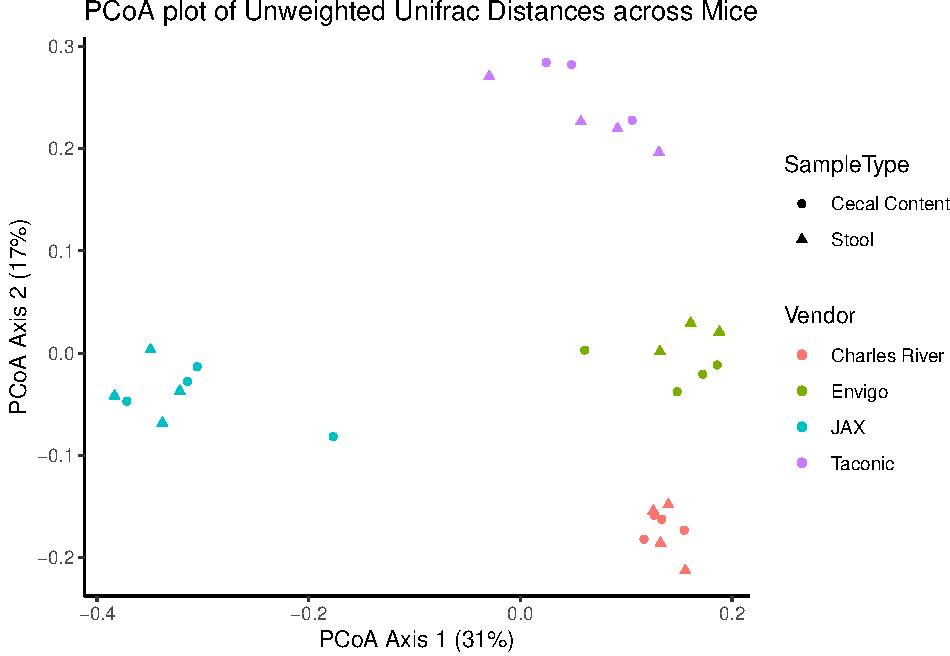
\includegraphics{final_paper_files/figure-latex/pcoa-ex-1.pdf}
\caption{\label{fig:pcoa-ex}PCoA plot of microbiota distances between mice}
\end{figure}

In Figure \ref{fig:pcoa-ex}, the PCoA plot was created from the
microbiota distance matrix for each mouse (two points per mouse, since
the microbiota was sampled in the cecum as well as in the stool). As
shown on the axes, the first PCoA Axis explains 31\% of the variance in
the original distance matrix. Creating a PCoA plot allows for a quick
and relatively simple way to visualize high-dimensional data to inform
future decisions on machine learning. From this plot, it is interesting
to note the separation of the different mice microbiota samples based on
where the mice were bought.

\section{t-SNE}\label{t-sne}

Another commonly used dimensionality reduction technique is
t-Distributed Stochastic Neighbor Embedding (t-SNE)
\citep{maaten2008visualizing}, which is a type of manifold learning.
t-SNE starts by calculating pairwise distances in the high-dimensional
space and using that information to calculate probabilities of a point
being next to each other \citep{tsnejs}. The method then randomly maps
the points onto a two-dimensional space and attempts to move the points
-- so that the probabilities of being next to the other points is
similar to the original probabilities in the high-dimensional space
\citep{tsnejs}. While a powerful technique, there are important caveats
when compared to techniques such as PCA. The usage of random placing and
probability-based calculations mean that when each time t-SNE is run,
the result is slightly different (unlike in PCA or PCoA where each run
is guaranteed to be the same). Furthermore, different settings in
determining the calculation of conditional probabilities can impact the
final outcome of the two-dimensional mapping.

\subsection{t-SNE example}\label{t-sne-example}

\begin{Shaded}
\begin{Highlighting}[]
\CommentTok{# create tsne model}
\NormalTok{do_tsne <-}\StringTok{ }\ControlFlowTok{function}\NormalTok{(dist_matrix, perp) \{}
  \KeywordTok{set.seed}\NormalTok{(}\DecValTok{9}\NormalTok{)}
\NormalTok{  tsne_model <-}\StringTok{ }\KeywordTok{Rtsne}\NormalTok{(}\KeywordTok{as.matrix}\NormalTok{(dist_matrix),}
                      \DataTypeTok{check_duplicates =} \OtherTok{FALSE}\NormalTok{,}
                      \DataTypeTok{is_distance =} \OtherTok{TRUE}\NormalTok{,}
                      \DataTypeTok{pca =} \OtherTok{FALSE}\NormalTok{,}
                      \DataTypeTok{perplexity =}\NormalTok{ perp,}
                      \DataTypeTok{theta =} \FloatTok{0.5}\NormalTok{,}
                      \DataTypeTok{dims =} \DecValTok{2}\NormalTok{)}

  \KeywordTok{return}\NormalTok{(}\KeywordTok{as.data.frame}\NormalTok{(tsne_model}\OperatorTok{$}\NormalTok{Y))}
\NormalTok{\}}

\NormalTok{df_tsne <-}\StringTok{ }\KeywordTok{do_tsne}\NormalTok{(uu, }\DecValTok{1}\NormalTok{) }\OperatorTok
\StringTok{  }\KeywordTok{mutate}\NormalTok{(}\DataTypeTok{perp =} \DecValTok{1}\NormalTok{) }\OperatorTok
\StringTok{  }\KeywordTok{cbind}\NormalTok{(s_vendor)}

\ControlFlowTok{for}\NormalTok{ (i }\ControlFlowTok{in} \KeywordTok{c}\NormalTok{(}\DecValTok{2}\OperatorTok{:}\DecValTok{9}\NormalTok{)) \{}
\NormalTok{  df <-}\StringTok{ }\KeywordTok{do_tsne}\NormalTok{(uu, i) }\OperatorTok
\StringTok{    }\KeywordTok{mutate}\NormalTok{(}\DataTypeTok{perp =}\NormalTok{ i) }\OperatorTok
\StringTok{    }\KeywordTok{cbind}\NormalTok{(s_vendor)}
  
\NormalTok{  df_tsne <-}\StringTok{ }\KeywordTok{rbind}\NormalTok{(df_tsne, df)}
\NormalTok{\}}

\KeywordTok{ggplot}\NormalTok{(df_tsne, }\KeywordTok{aes}\NormalTok{(}\DataTypeTok{x =}\NormalTok{ V1, }\DataTypeTok{y =}\NormalTok{ V2, }\DataTypeTok{color =}\NormalTok{ Vendor)) }\OperatorTok{+}
\StringTok{  }\KeywordTok{geom_point}\NormalTok{() }\OperatorTok{+}
\StringTok{  }\KeywordTok{labs}\NormalTok{(}\DataTypeTok{title =} \StringTok{"t-SNE Plot on Unweighted UniFrac Distances across Mice"}\NormalTok{,}
       \DataTypeTok{subtitle =} \StringTok{"With varying perplexity settings"}\NormalTok{,}
       \DataTypeTok{x =} \StringTok{"t-SNE Axis 1"}\NormalTok{,}
       \DataTypeTok{y =} \StringTok{"t-SNE Axis 2"}\NormalTok{) }\OperatorTok{+}
\StringTok{  }\KeywordTok{theme_bw}\NormalTok{() }\OperatorTok{+}
\StringTok{  }\KeywordTok{facet_wrap}\NormalTok{(}\OperatorTok{~}\StringTok{ }\NormalTok{perp, }\DataTypeTok{scales =} \StringTok{"free"}\NormalTok{)}
\end{Highlighting}
\end{Shaded}

\begin{figure}
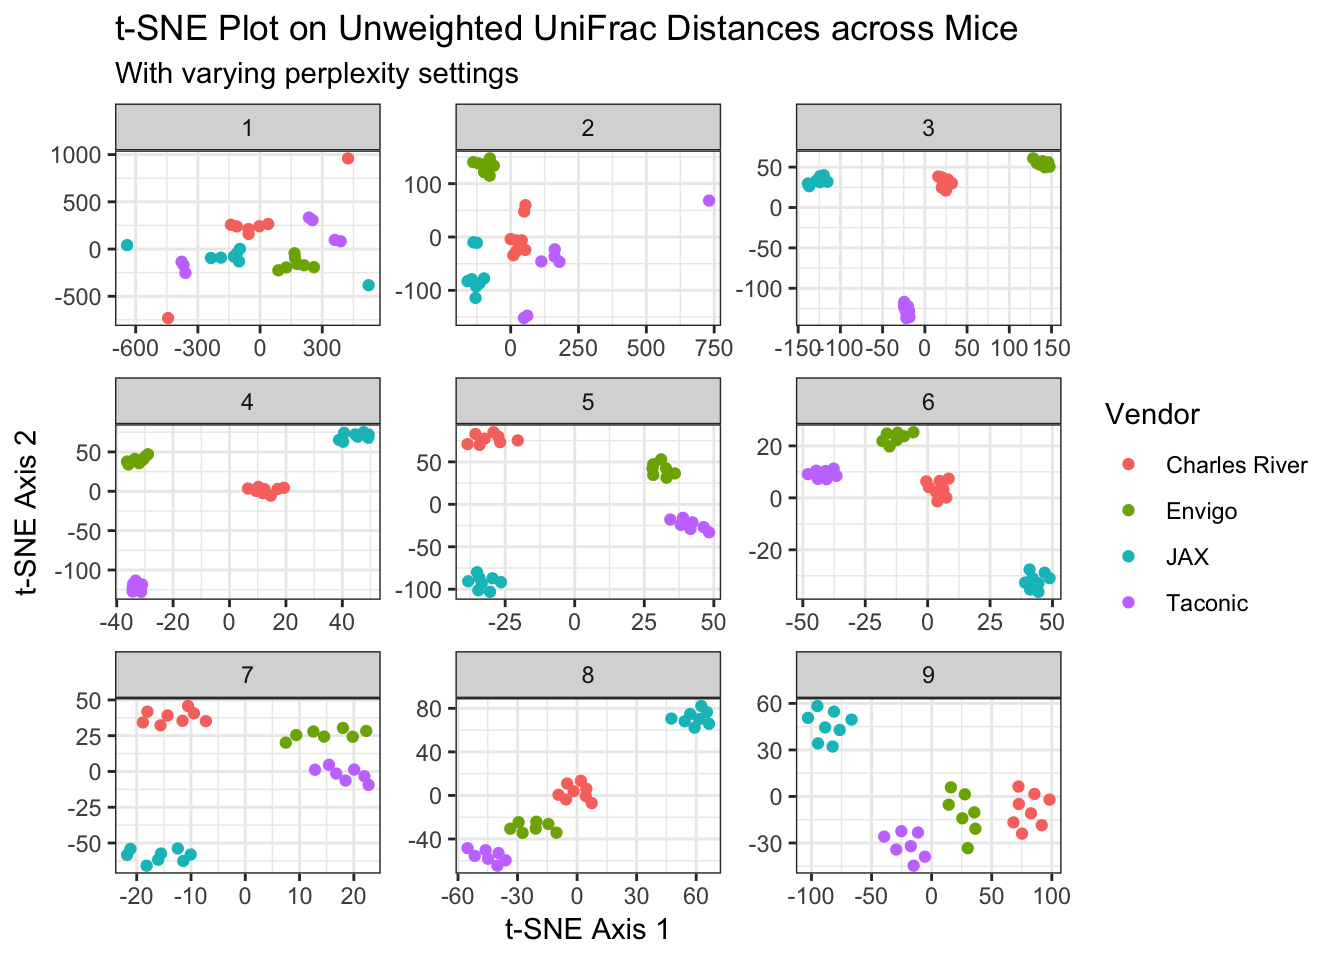
\includegraphics[width=1\linewidth]{final_paper_files/figure-latex/tsne-ex-1} \caption{t-SNE plot of microbiota distances between mice}\label{fig:tsne-ex}
\end{figure}

In Figure \ref{fig:tsne-ex}, t-SNE analysis was done on the same
distance matrix as in Figure \ref{fig:pcoa-ex} to transform into a
two-dimensional space. As with PCoA, one can see the differential
clustering by vendor. As mentioned in the previous paragraph, t-SNE
results can change based on the different settings. Figure
\ref{fig:tsne-ex} demonstrates how changing the \texttt{perplexity} can
impact the final result (number in gray bar indicates the perplexity for
that subplot).

\section{Other dimensionality reduction
techniques}\label{other-dimensionality-reduction-techniques}

PCA, PCoA, and t-SNE are common techniques used for dimensionality
reduction, but there are other methods that may perform better in
different contexts. For instance, a recent paper describes a new
technique similar to t-SNE for single-cell RNA sequencing called uniform
approximation and projection (UMAP) \citep{becht2018dimensionality}.
This method, like t-SNE, is considered a nonlinear dimensionality
reduction technique, as opposed to PCA where the usage of linear
combinations makes it a linear dimensionality reduction technique. While
there are multiple techniques available, the usage of PCA, PCoA, and
t-SNE are sufficient to demonstrate the machine learning techniques in
the next section.

\chapter{Supervised Learning}\label{sup_learn}

\section{Introduction to supervised
learning}\label{introduction-to-supervised-learning}

This section covers supervised learning techniques -- where the output
variables are already known. While there are many techniques available,
this paper will cover (1) regressions (multiple linear vs logistic vs
multinomial), (2) K-nearest neighbors, (3) decision trees, (4) random
forests, (5) deep learning, and (6) support vector machines. All of
these methods can be found in biomedical research papers, especially
those involving microbiome and next-generation sequencing data. Some of
these methods will include the code implementation, whereas others will
have only a description due to either data or paper restraints.

\section{Regressions}\label{regressions}

Regression is one of the simple (but still powerful) forms of supervised
learning. In brief, regression is an attempt to understand the
relationship between the input and output \citep{shalizi}. A linear
regression (commonly seen in papers with a plot, a regression line, a
\(r^2\) value, and a p-value) establishes a line with the lowest mean
squared error (distance between the data points and the line). The
\(r^2\) value, also known as the coefficient of determination, describes
how much of the variation in the output (typically the y-axis variable)
is explained by the input (typically the x-axis variable). As mentioned
in the background, the bias-variance tradeoff plays a role here as the
ability to predict an output is determined by the mean squared error (or
an equivalent measure) \citep{shalizi}.

\subsection{Linear regression example}\label{linear-regression-example}

\begin{Shaded}
\begin{Highlighting}[]
\NormalTok{aa <-}\StringTok{ }\KeywordTok{readRDS}\NormalTok{(}\StringTok{"data/aa.rds"}\NormalTok{)}
\NormalTok{mice <-}\StringTok{ }\KeywordTok{readRDS}\NormalTok{(}\StringTok{"data/mice.rds"}\NormalTok{)}

\NormalTok{lr_df <-}\StringTok{ }\NormalTok{aa }\OperatorTok
\StringTok{  }\KeywordTok{filter}\NormalTok{(Tissue }\OperatorTok{==}\StringTok{ "Stool"}\NormalTok{) }\OperatorTok
\StringTok{  }\KeywordTok{select}\NormalTok{(MouseID, Tissue, Metabolite, ConcentrationNZ)}

\NormalTok{lr_his_df <-}\StringTok{ }\NormalTok{lr_df }\OperatorTok
\StringTok{  }\KeywordTok{filter}\NormalTok{(Metabolite }\OperatorTok{==}\StringTok{ "Glycine"}\NormalTok{) }\OperatorTok
\StringTok{  }\KeywordTok{mutate}\NormalTok{(}\DataTypeTok{Glycine =}\NormalTok{ ConcentrationNZ) }\OperatorTok
\StringTok{  }\KeywordTok{select}\NormalTok{(MouseID, Tissue, Glycine) }\OperatorTok
\StringTok{  }\KeywordTok{mutate}\NormalTok{(}\DataTypeTok{y =} \OtherTok{NA}\NormalTok{,}
         \DataTypeTok{meta_comp =} \OtherTok{NA}\NormalTok{)}

\NormalTok{lr_g_df <-}\StringTok{ }\NormalTok{lr_his_df}

\NormalTok{lr_df <-}\StringTok{ }\NormalTok{lr_df }\OperatorTok
\StringTok{  }\KeywordTok{filter}\NormalTok{(Metabolite }\OperatorTok{!=}\StringTok{ "Glycine"}\NormalTok{)}

\NormalTok{uniq_meta <-}\StringTok{ }\KeywordTok{unique}\NormalTok{(lr_df}\OperatorTok{$}\NormalTok{Metabolite)}
\ControlFlowTok{for}\NormalTok{ (m }\ControlFlowTok{in}\NormalTok{ uniq_meta) \{}
\NormalTok{  df <-}\StringTok{ }\NormalTok{lr_df }\OperatorTok
\StringTok{    }\KeywordTok{filter}\NormalTok{(Metabolite }\OperatorTok{==}\StringTok{ }\NormalTok{m) }\OperatorTok
\StringTok{    }\KeywordTok{mutate}\NormalTok{(}\DataTypeTok{Glycine =}\NormalTok{ lr_his_df}\OperatorTok{$}\NormalTok{Glycine,}
           \DataTypeTok{y =}\NormalTok{ ConcentrationNZ,}
           \DataTypeTok{meta_comp =}\NormalTok{ Metabolite) }\OperatorTok
\StringTok{    }\KeywordTok{select}\NormalTok{(., }\OperatorTok{-}\NormalTok{ConcentrationNZ, }\OperatorTok{-}\NormalTok{Metabolite)}
  
\NormalTok{  lr_g_df <-}\StringTok{ }\KeywordTok{rbind}\NormalTok{(lr_g_df, df)}
\NormalTok{\}}

\NormalTok{lr_g_df <-}\StringTok{ }\NormalTok{lr_g_df }\OperatorTok\StringTok{ }\KeywordTok{filter}\NormalTok{(}\OperatorTok{!}\KeywordTok{is.na}\NormalTok{(meta_comp))}

\KeywordTok{ggplot}\NormalTok{(lr_g_df, }\KeywordTok{aes}\NormalTok{(}\DataTypeTok{x =}\NormalTok{ Glycine, }\DataTypeTok{y =}\NormalTok{ y)) }\OperatorTok{+}
\StringTok{  }\KeywordTok{geom_point}\NormalTok{(}\DataTypeTok{alpha =} \FloatTok{0.75}\NormalTok{) }\OperatorTok{+}
\StringTok{  }\KeywordTok{geom_smooth}\NormalTok{(}\DataTypeTok{method =} \StringTok{"lm"}\NormalTok{, }\DataTypeTok{se =} \OtherTok{FALSE}\NormalTok{) }\OperatorTok{+}
\StringTok{  }\KeywordTok{theme_bw}\NormalTok{() }\OperatorTok{+}
\StringTok{  }\KeywordTok{labs}\NormalTok{(}\DataTypeTok{title =} \StringTok{"Amino acid comparisons in stool"}\NormalTok{,}
    \DataTypeTok{subtitle =} \StringTok{"Glycine concentration vs other amino acids"}\NormalTok{,}
    \DataTypeTok{x =} \StringTok{"Glycine concentration"}\NormalTok{,}
    \DataTypeTok{y =} \StringTok{"Other amino acid concentration"}\NormalTok{) }\OperatorTok{+}
\StringTok{  }\KeywordTok{facet_wrap}\NormalTok{(}\OperatorTok{~}\StringTok{ }\NormalTok{meta_comp, }\DataTypeTok{ncol =} \DecValTok{3}\NormalTok{, }\DataTypeTok{scales =} \StringTok{"free"}\NormalTok{)}
\end{Highlighting}
\end{Shaded}

\begin{figure}
\centering
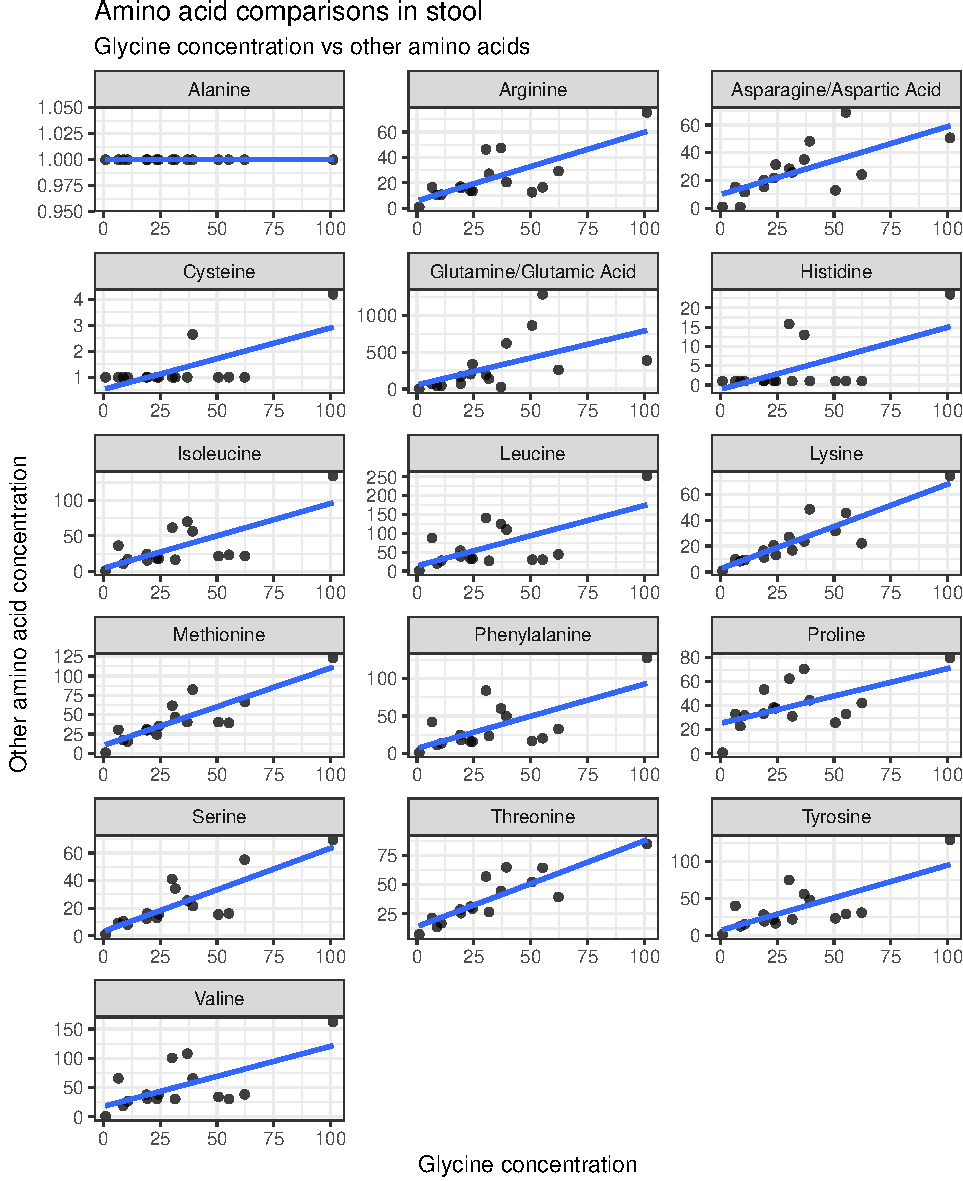
\includegraphics{final_paper_files/figure-latex/linreg-ex-1.pdf}
\caption{\label{fig:linreg-ex}Linear regression example}
\end{figure}

In Figure \ref{fig:linreg-ex}, metabolomic data was used due to the
restraints inherent to regression functions. Amino acid concentrations
were measured from stool samples. Glycine concentrations were then
compared with the other amino acids and a linear regression line was
drawn. From looking at how well the lines can represent the data points,
this graph is meant to demonstrate that some data, but not all, may work
well with a linear regression model. Even though linear regression may
be simple, it can be useful (i.e.~for the relationship between glycine
and lycine) or not as informative (i.e.~for the relationship between
glycine and histidine).

There are many types of regressions that are extensions of linear
regression\footnote{A useful resource for understanding regressions and
  other statistical topics is Pennsylvania State University's online
  documentation for their statistic courses. For example, STAT 504
  covers multinomial logistic regression and can be found at this link
  \url(\url{https://onlinecourses.science.psu.edu/stat504/node/172/}).}.
For instance, a multilinear regression factors in more than one input
variable to predict an output variable. Logistic regression is common in
the biological sciences when trying to analyze a dependent variable that
has a binary output (i.e. \(y = 0\) or \(y = 1\)) \citep{shalizi}. This
type of regression calculates the probability of \(y = 1\), as a
function of the independent variables. As such, a probability of greater
or equal to 0.5 will result in a prediction that \(y = 1\), otherwise it
will predict \(y = 0\). Multinomial regression (also known as polytomous
regression) builds on the same principles as logistic regression. The
main difference is that multinomial regression works for a dependent
variable that has more than two categories (i.e. \(y = 0\), \(y = 1\),
or \(y = 2\)).

\section{K-nearest neighbors (KNN)}\label{k-nearest-neighbors-knn}

KNN is a type of regression which takes into the account the distance
between points, hence its name \citep{shalizi}. This algorithm
calculates the distance between data points and a new data point of
interest (will be referred to as the query) to predict its
classification \citep{knn}. Of the \(k\) (a positive integer that is
less than the number of original data points) data points that are
closest to the query, the algorithm will then return the mode or mean of
the classifications of those data points (which is already known)
\citep{knn}. The thought is that the samples with the closest distances
to the query are likely to have the same classification, which would be
the predicted output for the query \citep{knn}. KNN falls under the
category of a linear smoother in creating a regression curve that is
smooth and close to the actual mean, when \(k\) is increased
\citep{shalizi}. The choosing of \(k\) for optimal KNN performance is
important due to the bias-variance tradeoff but will not be discussed in
this paper due to paper length restraints \citep{shalizi}.

\subsection{KNN example}\label{knn-example}

\begin{Shaded}
\begin{Highlighting}[]
\NormalTok{knn_df <-}\StringTok{ }\NormalTok{pc_df_uu }\OperatorTok
\StringTok{  }\KeywordTok{select}\NormalTok{(Vendor, Axis.}\DecValTok{1}\NormalTok{, Axis.}\DecValTok{2}\NormalTok{)}

\NormalTok{run_knn <-}\StringTok{ }\ControlFlowTok{function}\NormalTok{(k) \{}
\NormalTok{  res <-}\StringTok{ }\KeywordTok{c}\NormalTok{()}
  
  \ControlFlowTok{for}\NormalTok{ (i }\ControlFlowTok{in} \KeywordTok{c}\NormalTok{(}\DecValTok{1}\OperatorTok{:}\DecValTok{100}\NormalTok{)) \{}
\NormalTok{    df <-}\StringTok{ }\NormalTok{knn_df }\OperatorTok
\StringTok{      }\KeywordTok{mutate}\NormalTok{(}\DataTypeTok{trial =} \KeywordTok{sample}\NormalTok{(}\DecValTok{2}\NormalTok{, }\KeywordTok{n}\NormalTok{(), }\DataTypeTok{replace =} \OtherTok{TRUE}\NormalTok{, }\DataTypeTok{prob =} \KeywordTok{c}\NormalTok{(}\FloatTok{0.67}\NormalTok{, }\FloatTok{0.33}\NormalTok{)))}
  
\NormalTok{    knn_train <-}\StringTok{ }\NormalTok{df }\OperatorTok
\StringTok{      }\KeywordTok{filter}\NormalTok{(trial }\OperatorTok{==}\StringTok{ }\DecValTok{1}\NormalTok{)}
    
\NormalTok{    knn_test <-}\StringTok{ }\NormalTok{df }\OperatorTok
\StringTok{      }\KeywordTok{filter}\NormalTok{(trial }\OperatorTok{==}\StringTok{ }\DecValTok{2}\NormalTok{)}
    
\NormalTok{    knn_prd <-}\StringTok{ }\KeywordTok{knn}\NormalTok{(}\DataTypeTok{train =}\NormalTok{ knn_train }\OperatorTok\StringTok{ }\KeywordTok{select}\NormalTok{(., }\OperatorTok{-}\NormalTok{Vendor),}
                   \DataTypeTok{test =}\NormalTok{ knn_test }\OperatorTok\StringTok{ }\KeywordTok{select}\NormalTok{(., }\OperatorTok{-}\NormalTok{Vendor),}
                   \DataTypeTok{cl =}\NormalTok{ knn_train}\OperatorTok{$}\NormalTok{Vendor,}
                   \DataTypeTok{k =}\NormalTok{ k)}
    
\NormalTok{    prop <-}\StringTok{ }\KeywordTok{sum}\NormalTok{((knn_test}\OperatorTok{$}\NormalTok{Vendor }\OperatorTok{==}\StringTok{ }\NormalTok{knn_prd) }\OperatorTok{==}\StringTok{ }\OtherTok{TRUE}\NormalTok{,}
                \DataTypeTok{na.rm =} \OtherTok{TRUE}\NormalTok{) }\OperatorTok{/}\StringTok{ }\KeywordTok{length}\NormalTok{(knn_prd)}
\NormalTok{    res <-}\StringTok{ }\KeywordTok{c}\NormalTok{(res, prop)}
\NormalTok{  \}}
  
  \KeywordTok{return}\NormalTok{(res)}
\NormalTok{\}}

\NormalTok{res_df <-}\StringTok{ }\KeywordTok{data.frame}\NormalTok{(}\DataTypeTok{k =} \KeywordTok{c}\NormalTok{(}\KeywordTok{rep}\NormalTok{(}\DecValTok{3}\NormalTok{, }\DecValTok{100}\NormalTok{), }\KeywordTok{rep}\NormalTok{(}\DecValTok{4}\NormalTok{, }\DecValTok{100}\NormalTok{), }\KeywordTok{rep}\NormalTok{(}\DecValTok{5}\NormalTok{, }\DecValTok{100}\NormalTok{)),}
                     \DataTypeTok{accuracy =} \KeywordTok{c}\NormalTok{(}\KeywordTok{run_knn}\NormalTok{(}\DecValTok{3}\NormalTok{),}
                                  \KeywordTok{run_knn}\NormalTok{(}\DecValTok{4}\NormalTok{),}
                                  \KeywordTok{run_knn}\NormalTok{(}\DecValTok{5}\NormalTok{)))}

\KeywordTok{ggplot}\NormalTok{(res_df, }\KeywordTok{aes}\NormalTok{(}\DataTypeTok{x =}\NormalTok{ accuracy, }\DataTypeTok{fill =} \KeywordTok{as.factor}\NormalTok{(k), }\DataTypeTok{color =} \KeywordTok{as.factor}\NormalTok{(k))) }\OperatorTok{+}
\StringTok{  }\KeywordTok{geom_density}\NormalTok{(}\DataTypeTok{alpha =} \FloatTok{0.6}\NormalTok{) }\OperatorTok{+}
\StringTok{  }\KeywordTok{labs}\NormalTok{(}\DataTypeTok{title =} \StringTok{"KNN Regression with Varied k values"}\NormalTok{,}
       \DataTypeTok{color =} \StringTok{"k value"}\NormalTok{,}
       \DataTypeTok{fill =} \StringTok{"k value"}\NormalTok{,}
       \DataTypeTok{x =} \StringTok{"Prediction accuracy"}\NormalTok{,}
       \DataTypeTok{y =} \StringTok{"Density"}\NormalTok{) }\OperatorTok{+}
\StringTok{  }\KeywordTok{theme_bw}\NormalTok{()}
\end{Highlighting}
\end{Shaded}

\begin{figure}
\centering
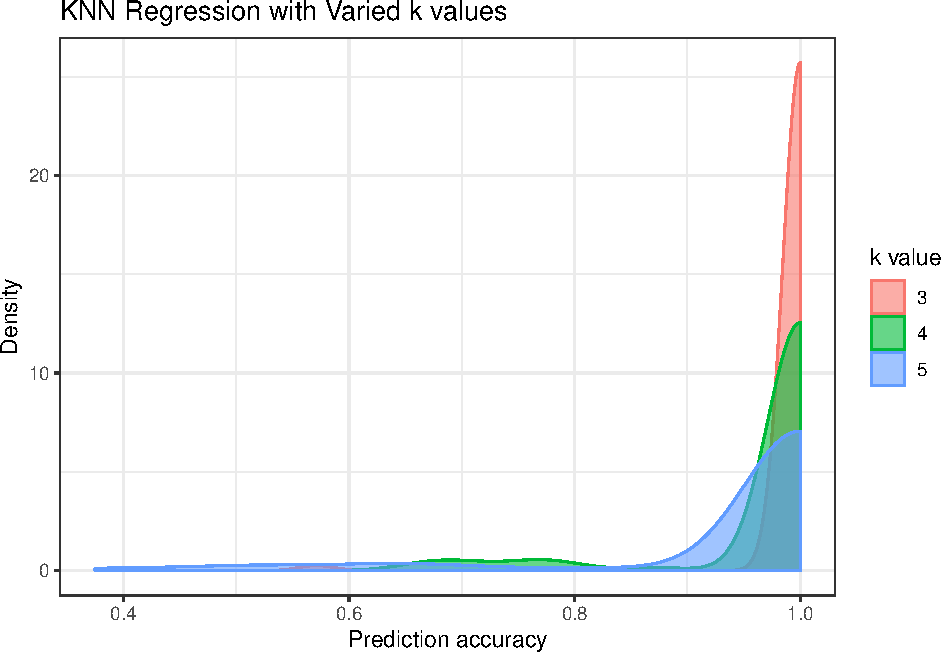
\includegraphics{final_paper_files/figure-latex/knn-ex-1.pdf}
\caption{\label{fig:knn-ex}KNN example}
\end{figure}

In Figure \ref{fig:knn-ex}, the KNN method was applied to the PCoA
transformed data points (as seen in Figure \ref{fig:pcoa-ex}). The data
was split into a training and a testing dataset in order to see how well
the KNN could predict vendor with different values of \(k\). The graph
demonstrates how different values of \(k\) can impact prediction
accuracy.

\section{Decision trees}\label{decision-trees}

Decision trees fall into the category of nonparametric supervised
learning methods, meaning that it does not depend on the distribution of
the variables. In brief, decision trees separate the data based on
different variables and construct a tree for predicting the final
classification. The algorithm aims to create the smallest tree (requires
the least number of variables) that increases information gain
(selecting variables that can split the data into two subsets that are
individually homogenous) \citep{dt}.

\begin{Shaded}
\begin{Highlighting}[]
\NormalTok{aa_dt_df <-}\StringTok{ }\NormalTok{lr_df }\OperatorTok
\StringTok{  }\KeywordTok{left_join}\NormalTok{(}\KeywordTok{select}\NormalTok{(mice, MouseID, Vendor), }\DataTypeTok{by =} \StringTok{"MouseID"}\NormalTok{) }\OperatorTok
\StringTok{  }\KeywordTok{mutate}\NormalTok{(}\DataTypeTok{Metabolite =} \KeywordTok{gsub}\NormalTok{(}\StringTok{"[/ ]"}\NormalTok{, }\StringTok{"_"}\NormalTok{, Metabolite)) }\OperatorTok
\StringTok{  }\KeywordTok{spread}\NormalTok{(Metabolite, ConcentrationNZ) }\OperatorTok
\StringTok{  }\KeywordTok{mutate}\NormalTok{(}\DataTypeTok{Vendor =} \KeywordTok{as.factor}\NormalTok{(Vendor))}

\NormalTok{aa_lbls <-}\StringTok{ }\KeywordTok{colnames}\NormalTok{(aa_dt_df)[}\DecValTok{5}\OperatorTok{:}\KeywordTok{length}\NormalTok{(aa_dt_df)]}

\NormalTok{tree_fm <-}\StringTok{ }\KeywordTok{as.formula}\NormalTok{(}\KeywordTok{paste}\NormalTok{(}\StringTok{"Vendor ~ "}\NormalTok{, }\KeywordTok{paste}\NormalTok{(aa_lbls, }\DataTypeTok{collapse =} \StringTok{" + "}\NormalTok{), }\DataTypeTok{sep =} \StringTok{""}\NormalTok{))}

\NormalTok{tree_res <-}\StringTok{ }\KeywordTok{tree}\NormalTok{(tree_fm, }\DataTypeTok{data =}\NormalTok{ aa_dt_df)}

\KeywordTok{plot}\NormalTok{(tree_res)}
\KeywordTok{text}\NormalTok{(tree_res)}
\end{Highlighting}
\end{Shaded}

\begin{figure}
\centering
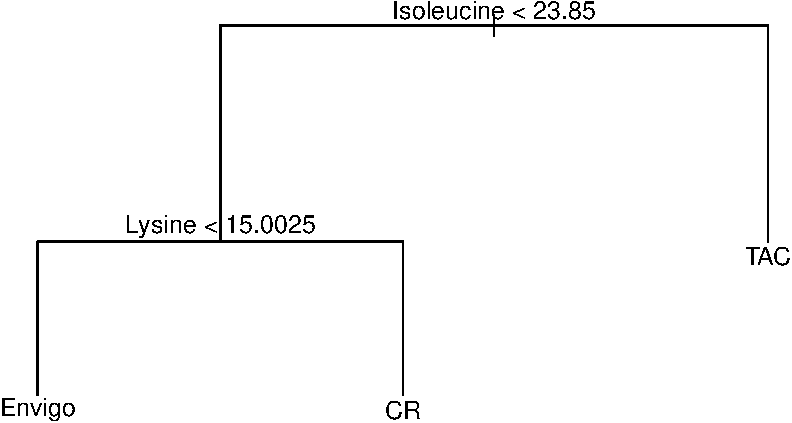
\includegraphics{final_paper_files/figure-latex/dt-ex-1.pdf}
\caption{\label{fig:dt-ex}Decision tree example using amino acid
concentrations to predict vendor}
\end{figure}

In Figure \ref{fig:dt-ex}, the decision tree method was applied to the
metabolite dataset (as seen in Figure \ref{fig:linreg-ex}). All the
amino acids detected were used to try to classify the samples by vendor.
As seen in the result, isoleucine levels \(\geq\) 23.85 can predict
samples from TAC. Proceeding down the decision tree can further separate
the samples by using lysine levels.

\section{Random forests}\label{random-forests}

This method is an extension of decision trees with the same aim of
predicting the final classification for a data point
\citep{breiman2001random, liaw2002classification}. The algorithm starts
by randomly grabbing a chunk of data from the dataset (called the
training data) and creating a single decision tree. It will then test
the accuracy of that tree by using it on the data that was not initially
used for constructing the tree. The algorithm then repeats this process
by grabbing another random chunk of data and constructing another tree.
By repeating this process multiple times, the algorithm will create a
large number of decision trees, hence the term random forests. Once a
random forest is established, the trees will take in new data and will
each generate their own prediction of what the classification is. The
algorithm will select the most common classification and return that as
the predicted classification for the new data.

\begin{Shaded}
\begin{Highlighting}[]
\NormalTok{forest_res <-}\StringTok{ }\KeywordTok{randomForest}\NormalTok{(tree_fm, }\DataTypeTok{data =}\NormalTok{ aa_dt_df)}

\KeywordTok{importance}\NormalTok{(forest_res)}
\end{Highlighting}
\end{Shaded}

\begin{verbatim}
##                          MeanDecreaseGini
## Arginine                       0.52426159
## Asparagine_Aspartic_Acid       0.48782994
## Cysteine                       0.08388865
## Glutamine_Glutamic_Acid        0.79407455
## Histidine                      0.10707186
## Isoleucine                     1.33005098
## Leucine                        0.90613227
## Lysine                         1.01425911
## Methionine                     1.16218851
## Phenylalanine                  0.97286201
## Proline                        0.54284661
## Serine                         0.63527573
## Threonine                      0.73175700
## Tyrosine                       1.23192239
## Valine                         0.75157881
\end{verbatim}

The output of random forests includes its ability to accurately predict
the samples as well as the relative importance of the independent
variables used to construct the forest. Isoleucine is identified as an
important separator, which supports the finding in Figure
\ref{fig:dt-ex}.

\section{Neural networks (NN)}\label{neural-networks-nn}

NN and the field of deep learning, like many of the methods mentioned
here, are topics that can each be written about in their own paper (or
book) \citep{Goodfellow-et-al-2016}. This subsection only serves to
briefly introduce this and include resources for further exploration.
NNs, in short, aim to mimic how neurons act\footnote{The developers of a
  software package called TensorFlow (an open-source package for running
  neural networks) have also created an interactive simulation of neural
  networks at this link
  (\url(\url{https://playground.tensorflow.org/})).}. The input of data
(analogous to neurotransmitters) results in an output (analogous to
whether or not the neuron fires). The beauty of neural networks lies
within its name, where multiple layers of neurons are connected with
each other. NNs have impressive predictive capabilities by learning from
vast amounts of data. For instance, NNs can be trained to recognize
objects in pictures, to recognize handwriting, and other tasks that
strike at the core of deep learning
\citep{Nielsen-2015, Goodfellow-et-al-2016}. NN are increasingly present
in the biological sciences as research groups contribute towards large
and accessible databases, which present prime opportunities for the
development of neural networks to predict outputs such as treatment
outcomes \citep{snow1994artificial, kappen1993neural} and diagnoses
\citep{ercal1994neural, acharya2018deep, esteva2017dermatologist}.

\section{Support vector machines
(SVM)}\label{support-vector-machines-svm}

SVM is a popular method \citep{furey2000support, guyon2002gene} used for
classification in the biological sciences because of its ability to deal
with high dimensional data and to look at non-linear relationships. This
method searches for a hyperplane (in 2D: a line; in 3D: a plane, etc.)
that can separate the data points, which is determined by having the
largest average distance from each of the data points to the hyperplane
\citep{svmdata}. SVM employs a method called a kernel trick\footnote{This
  post
  (\url(\url{https://stats.stackexchange.com/questions/152897/how-to-intuitively-explain-what-a-kernel-is}))
  offers an explanation about how kernel tricks work.} to perceive data
points in different dimensional space in order to find the best
hyperplane \citep{svmdata}. After a hyperplane is identified, new data
points can be classified by which side they fall on the hyperplane.

\subsection{SVM example}\label{svm-example}

\begin{Shaded}
\begin{Highlighting}[]
\NormalTok{svm_df <-}\StringTok{ }\NormalTok{pc_df_uu }\OperatorTok
\StringTok{  }\KeywordTok{select}\NormalTok{(Vendor, Axis.}\DecValTok{1}\NormalTok{, Axis.}\DecValTok{2}\NormalTok{)}

\CommentTok{# get best model on cost}
\NormalTok{model_svms <-}\StringTok{ }\KeywordTok{tune}\NormalTok{(svm,}
                   \KeywordTok{as.factor}\NormalTok{(Vendor) }\OperatorTok{~}\StringTok{ }\NormalTok{.,}
                   \DataTypeTok{data =}\NormalTok{ svm_df,}
                   \DataTypeTok{kernel =} \StringTok{"radial"}\NormalTok{,}
                   \DataTypeTok{ranges =} \KeywordTok{list}\NormalTok{(}\DataTypeTok{cost =} \KeywordTok{c}\NormalTok{(}\FloatTok{0.001}\NormalTok{, }\FloatTok{0.01}\NormalTok{, }\FloatTok{0.1}\NormalTok{, }\DecValTok{1}\NormalTok{, }\DecValTok{5}\NormalTok{, }\DecValTok{10}\NormalTok{, }\DecValTok{100}\NormalTok{)))}

\CommentTok{# get parameters for best model}
\NormalTok{best_svm <-}\StringTok{ }\NormalTok{model_svms}\OperatorTok{$}\NormalTok{best.model}

\CommentTok{# predict based on SVM and plot}
\NormalTok{pred <-}\StringTok{ }\KeywordTok{predict}\NormalTok{(best_svm, svm_df, }\DataTypeTok{decision.values =} \OtherTok{TRUE}\NormalTok{)}
\KeywordTok{plot}\NormalTok{(best_svm, svm_df)}
\end{Highlighting}
\end{Shaded}

\begin{figure}
\centering
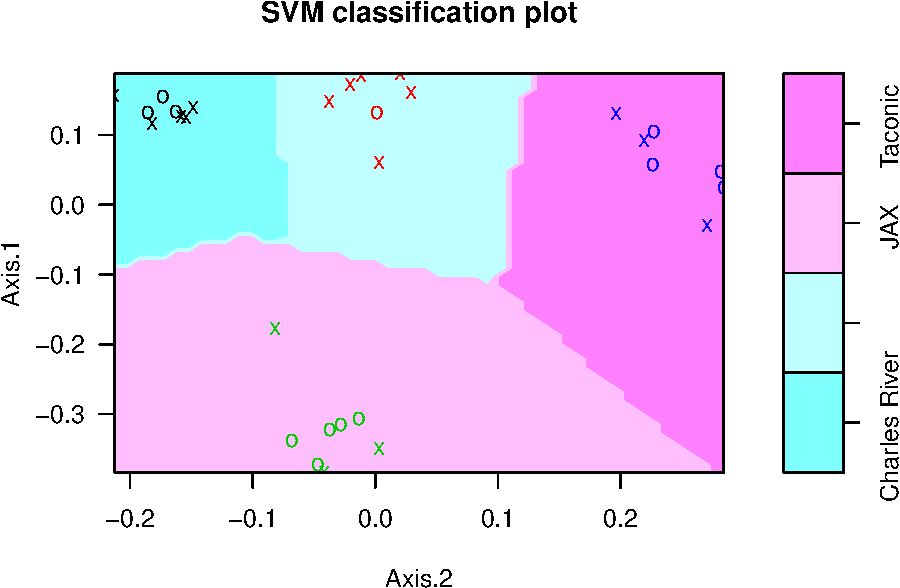
\includegraphics{final_paper_files/figure-latex/svm-ex-1.pdf}
\caption{\label{fig:svm-ex}SVM classification of unweighted UniFrac
distances}
\end{figure}

In Figure \ref{fig:svm-ex}, SVM was applied to the PCoA transformed
dataset (as seen in Figure \ref{fig:pcoa-ex}). If the data points from
Figure \ref{fig:pcoa-ex} are mirrored and then rotated, the points will
be the same as seen here in Figure \ref{fig:svm-ex}. Based on the
shading, it is interesting to note how SVM can demarcate areas
associated with different vendors in the PCoA space. These boundaries
are effective, at least for this dataset, in classifying the samples by
the correct vendor.

\chapter{Unsupervised Learning}\label{unsup_learn}

\section{Introduction to unsupervised
learning}\label{introduction-to-unsupervised-learning}

Unsupervised machine learning is arguably a more difficult task as the
classifications are not known \emph{a priori}. These methods use
clustering to discover ways that the data can be grouped. Techniques
mentioned above such as PCA, PCoA, and t-SNE can be useful in viewing
the data in a lower dimension and can be a good starting point for
unsupervised learning. This paper will cover 1) hierarchical clustering,
2) divisive clustering, and 3) hidden Markov models. As with the
supervised learning section, some of these methods will be only be
described while others will contain accompanying R code and graphics.

\section{Hierarchical agglomerative
clustering}\label{hierarchical-agglomerative-clustering}

This type of unsupervised learning can be seen from recent papers that
utilize heatmaps and have dendrograms drawn on either or both axes
\citep{buggert2018identification, byrd2017staphylococcus}. These
dendrograms are the final product of hierarchical clustering. Distance
measurements between each data point are used to cluster the data
points, which can then be portrayed as a binary tree (each branch point
separates into two children). In a hierarchical clustering dendrogram,
the similarities between two points can be assessed by looking at the
height of the first shared node (analogous to looking at the most recent
common ancestor in a phylogeny) \citep{cluster}. Hierarchical clustering
can provide insight on any underlying structure and can be useful when
accompanied with heatmaps to show clusters in a quantitative and
qualitative manner \citep{cluster}.

\section{Hierarchical divisive
clustering}\label{hierarchical-divisive-clustering}

Divisive clustering is a type of hierarchical clustering that differs
from agglomerative clustering by its approach in dividing the data.
Agglomerative clustering, as its name suggests, starts with the data
points as individual parts and starts grouping those together to create
the tree (as if drawing the tree from the branches to the root)
\citep{cluster}. Divisive clustering takes the opposite approach and
starts with all the data points in one group and divides that group to
create the tree (as if drawing the tree from root to the branches)
\citep{0521865719, cluster}. The advantage of divisive clustering is
that it takes into account how the data looks at a global perspective,
whereas agglomerative clustering loses that perspective when starting
with each data point as an individual \citep{cluster}.

Two of the methods to divide the first group for divisive clustering
include k-means and partitioning across medoids (PAM). While there are
significant differences between the two methods, the idea is similar in
which clusters are created based on the proximity to the closest
centroid (mean of a specific cluster of data points) or to the medoid (a
data point that is selected as the center of a cluster). The difficulty
for either method comes to choosing the value for \(k\), which is the
number of clusters that the scientist must assign \emph{a priori}. There
are multiple techniques for deciding \(k\), such as the sum of squares
method or the silhouette method.

\subsection{K-means example}\label{k-means-example}

\begin{Shaded}
\begin{Highlighting}[]
\NormalTok{do_kmeans <-}\StringTok{ }\ControlFlowTok{function}\NormalTok{(df, dist) \{}
\NormalTok{  df_kmeans <-}\StringTok{ }\NormalTok{df}
\NormalTok{  sum_sq <-}\StringTok{ }\KeywordTok{c}\NormalTok{()}
\NormalTok{  col_names <-}\StringTok{ }\KeywordTok{c}\NormalTok{()}
\NormalTok{  sil_width <-}\StringTok{ }\KeywordTok{c}\NormalTok{()}
\NormalTok{  iterations <-}\StringTok{ }\KeywordTok{c}\NormalTok{(}\DecValTok{2}\OperatorTok{:}\DecValTok{10}\NormalTok{)}
  
  \CommentTok{# run kmeans}
  \ControlFlowTok{for}\NormalTok{ (i }\ControlFlowTok{in}\NormalTok{ iterations) \{}
\NormalTok{    kmeans_model <-}\StringTok{ }\KeywordTok{kmeans}\NormalTok{(}\KeywordTok{scale}\NormalTok{(df), i)}
    
\NormalTok{    col_name <-}\StringTok{ }\KeywordTok{paste}\NormalTok{(}\StringTok{"cl_kmeans_"}\NormalTok{, i, }\DataTypeTok{sep =} \StringTok{""}\NormalTok{)}
\NormalTok{    col_names <-}\StringTok{ }\KeywordTok{c}\NormalTok{(col_names, col_name)}
    
\NormalTok{    df_kmeans[, col_name] <-}\StringTok{ }\NormalTok{kmeans_model}\OperatorTok{$}\NormalTok{cluster}
\NormalTok{    sum_sq <-}\StringTok{ }\KeywordTok{c}\NormalTok{(sum_sq, kmeans_model}\OperatorTok{$}\NormalTok{tot.withinss)}
    
\NormalTok{    sil <-}\StringTok{ }\KeywordTok{silhouette}\NormalTok{(kmeans_model}\OperatorTok{$}\NormalTok{cluster, dist)}
\NormalTok{    sil_width <-}\StringTok{ }\KeywordTok{c}\NormalTok{(sil_width, }\KeywordTok{summary}\NormalTok{(sil)}\OperatorTok{$}\NormalTok{avg.width)}
\NormalTok{  \}}
  
\NormalTok{  df_kmeans <-}\StringTok{ }\NormalTok{df_kmeans }\OperatorTok
\StringTok{    }\KeywordTok{gather_}\NormalTok{(}\StringTok{"k"}\NormalTok{, }\StringTok{"cluster"}\NormalTok{, col_names) }\OperatorTok
\StringTok{    }\KeywordTok{mutate}\NormalTok{(}\DataTypeTok{k =} \KeywordTok{gsub}\NormalTok{(}\StringTok{"^cl_kmeans_"}\NormalTok{, }\StringTok{""}\NormalTok{, k))}
  
  \CommentTok{# plot clustering}
\NormalTok{  p <-}\StringTok{ }\KeywordTok{ggplot}\NormalTok{(df_kmeans, }\KeywordTok{aes}\NormalTok{(}\DataTypeTok{x =}\NormalTok{ V1, }\DataTypeTok{y =}\NormalTok{ V2, }\DataTypeTok{color =} \KeywordTok{as.factor}\NormalTok{(cluster))) }\OperatorTok{+}
\StringTok{    }\KeywordTok{geom_point}\NormalTok{(}\DataTypeTok{alpha =} \FloatTok{0.5}\NormalTok{) }\OperatorTok{+}
\StringTok{    }\KeywordTok{labs}\NormalTok{(}\DataTypeTok{title =} \StringTok{"k-means clustering"}\NormalTok{,}
         \DataTypeTok{x =} \StringTok{"Axis 1"}\NormalTok{,}
         \DataTypeTok{y =} \StringTok{"Axis 2"}\NormalTok{,}
         \DataTypeTok{color =} \StringTok{"Cluster #"}\NormalTok{) }\OperatorTok{+}
\StringTok{    }\KeywordTok{theme_bw}\NormalTok{() }\OperatorTok{+}
\StringTok{    }\CommentTok{# scale_color_viridis(discrete = TRUE) +}
\StringTok{    }\KeywordTok{facet_wrap}\NormalTok{( }\OperatorTok{~}\StringTok{ }\KeywordTok{as.numeric}\NormalTok{(k))}
  
  \CommentTok{# look at sum of squares}
\NormalTok{  p2 <-}\StringTok{ }\KeywordTok{qplot}\NormalTok{(}\DataTypeTok{x =}\NormalTok{ iterations, }\DataTypeTok{y =}\NormalTok{ sum_sq) }\OperatorTok{+}
\StringTok{    }\KeywordTok{geom_point}\NormalTok{() }\OperatorTok{+}
\StringTok{    }\KeywordTok{labs}\NormalTok{(}\DataTypeTok{title =} \StringTok{"Which k to pick?"}\NormalTok{,}
         \DataTypeTok{subtitle =} \StringTok{"Sum of squares method"}\NormalTok{,}
         \DataTypeTok{x =} \StringTok{"k"}\NormalTok{,}
         \DataTypeTok{y =} \StringTok{"Total within sum of squares"}\NormalTok{) }\OperatorTok{+}
\StringTok{    }\KeywordTok{theme_bw}\NormalTok{()}
  
  \KeywordTok{return}\NormalTok{(}\KeywordTok{list}\NormalTok{(p, p2))}
\NormalTok{\}}
\end{Highlighting}
\end{Shaded}

\begin{Shaded}
\begin{Highlighting}[]
\NormalTok{rename_pc_df <-}\StringTok{ }\ControlFlowTok{function}\NormalTok{(df) \{}
\NormalTok{  df <-}\StringTok{ }\NormalTok{df }\OperatorTok
\StringTok{    }\KeywordTok{select}\NormalTok{(Axis.}\DecValTok{1}\NormalTok{, Axis.}\DecValTok{2}\NormalTok{) }\OperatorTok
\StringTok{    }\KeywordTok{rename}\NormalTok{(}\DataTypeTok{V1 =}\NormalTok{ Axis.}\DecValTok{1}\NormalTok{,}
           \DataTypeTok{V2 =}\NormalTok{ Axis.}\DecValTok{2}\NormalTok{)}
  
  \KeywordTok{return}\NormalTok{(df)}
\NormalTok{\}}

\NormalTok{graphs <-}\StringTok{ }\KeywordTok{do_kmeans}\NormalTok{(}\KeywordTok{rename_pc_df}\NormalTok{(pc_df_uu), uu)}

\NormalTok{graphs[[}\DecValTok{1}\NormalTok{]]}
\end{Highlighting}
\end{Shaded}

\begin{figure}
\centering
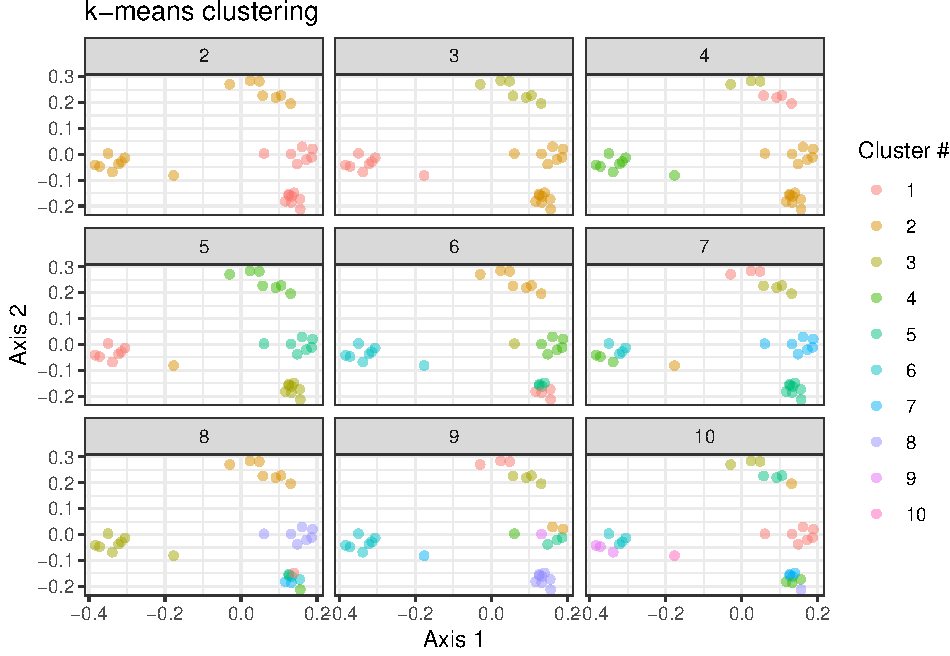
\includegraphics{final_paper_files/figure-latex/km-ex-1.pdf}
\caption{\label{fig:km-ex}Kmeans clustering with different k values}
\end{figure}

\begin{Shaded}
\begin{Highlighting}[]
\NormalTok{graphs[[}\DecValTok{2}\NormalTok{]]}
\end{Highlighting}
\end{Shaded}

\begin{figure}
\centering
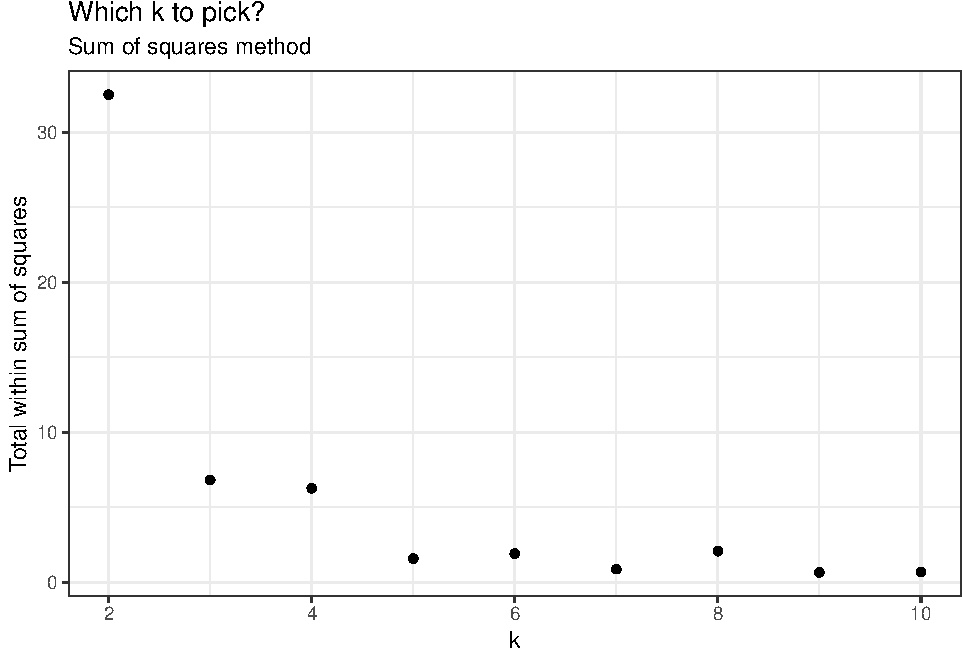
\includegraphics{final_paper_files/figure-latex/km-ex-ws-1.pdf}
\caption{\label{fig:km-ex-ws}Deciding which k to use}
\end{figure}

In Figure \ref{fig:km-ex}, this clustering was done on the same PCoA
transformed data for unweighted UniFrac distances between mice. The
value of \(k\) (indicated by number in the gray bar) was varied and then
graphed to show how the clusters appear (each cluster was assigned a
number). In Figure \ref{fig:km-ex-ws}, it is possible to use the
\texttt{total\ within\ sum\ of\ squares} measure to determine the best
\(k\) value. The points dip and start to progress in a flat trajectory
around \(k=4\), suggesting that \(k=4\) is the best \(k\) value for this
specific data.

\section{Hidden Markov models (HMM)}\label{hidden-markov-models-hmm}

A Markov model is a model that describes a system where state
transitions are random and are independent of past events
\citep{rabiner1986introduction, eddy2004hidden}. For example, Figure
\ref{fig:mm-fig} shows a two state Markov model. From state A, there is
a 30\% chance of going back to state A or a 70\% chance of going to
state B regardless of any previous transitions. This simple model can be
extended to multiple states with more transition weights. In HMMs, the
overall idea is similar but there can also be hidden states and weights.
HMMs are commonly used when studying nucleotide or amino acid sequences
\citep{eddy1998profile, eddy2004hidden}. Examples include sequence
alignment tools as well as the HMMER program \citep{finn2011hmmer},
which can take in an amino acid sequence and output proteins that are
related to your sequence of interest. Furthermore, HMMs have been used
for species-level and even strain-level identification for microbiome
studies via the HmmUFOtu program \citep{zheng2018hmmufotu}, developed
here at Penn.

\begin{figure}

{\centering 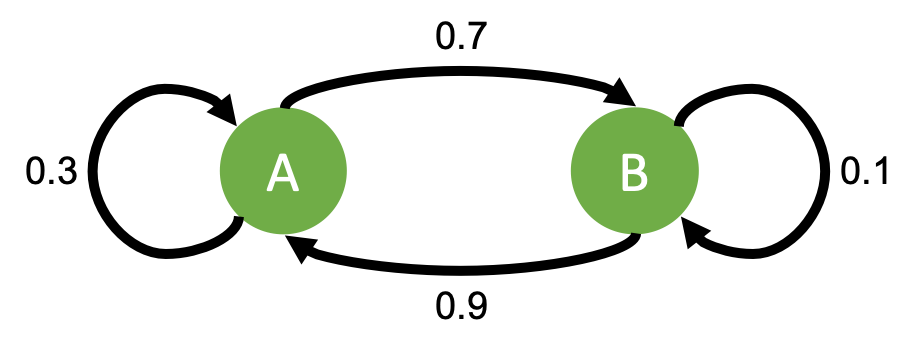
\includegraphics[width=0.35\linewidth]{fig/mm_fig} 

}

\caption{Simple HMM example}\label{fig:mm-fig}
\end{figure}

\chapter{Conclusion}\label{con}

The techniques mentioned in this paper are only a subset of the wide
spectrum of techniques that are being used and developed. These methods,
spanning from linear regression to hidden Markov models, are all context
dependent -- in terms of the data (i.e.~whether there is missing data,
categorical vs continuous, etc.) and the hypotheses that one is trying
to answer. Choosing the ``right'' method is not an easy task and must
also take into account what has been done in the field. Furthermore, the
increased communication and synergy between research fields has allowed
for novel applications of a field's existing tools/methods to a
different field.

During a discussion one day, my class mentor and I referred to a saying
that ``all models are wrong; but some are less wrong than
others''\footnote{This is a modified version of George E.P. Box's quote
  from two of his papers: ``All models are wrong but some are useful''
  \citep{box1976science, box1979robustness}.}. While it may seem
unfortunate, this quote has some validity. For instance, the human eye
and brain can distinguish clusters and grouping that are difficult for
computers to recapitulate. In the PCoA plot that was used in this paper,
we are capable of quickly discerning the groups manually by eye.
However, using our own eyes leaves room for error and potential
inconsistencies across people. As such, my view of machine learning is
as a way of emulating and improving on what humans can do -- lending
itself to the idea of ``learning''.

The benefits of machine learning methods far outweigh the limitations.
Machine learning can process data on a larger and faster scale than we
can, especially in higher dimensional spaces with many data points.
These methods are capable of processing and understanding the underlying
relationships within data -- especially from sources like
next-generation sequencing. Developing new techniques as well as
improving the accessibility of existing techniques to the larger
scientific community will create opportunities for unique questions to
be answered.

\bibliography{book.bib,packages.bib}


\end{document}
